\chapter{Motivations}
\minitoc%
\pagenumbering{arabic}
\setcounter{page}{1}

Dans le cadre de ce stage, les données que l'on traite sont des données du secteur de l'énergie, et plus particulièrement des données de production électrique. On dispose ainsi de plusieurs éoliennes identifiées par le tag "id\_[identifiant de l'éolienne]" dont l'énergie produite est mesurée toutes les demies heures, et ce pendant 4 ans (de de 2014 à 2017).
Cette énergie produite est dénommée la courbe de charge (que l'on abbrégera par \textbf{CDC} par la suite). Il est cependant plus utile de s'intéresser au facteur de charge (ou \textbf{FDC}) qui est défini comme
$\displaystyle\textsf{Facteur de Charge} = \frac{\textsf{Courbe de Charge}}{\textsf{Puissance Installée}}$.
On en déduit que \textbf{FDC} doit nécessairement être compris entre 0 et 1. C'est entre autre aussi une manière de détecter des anomalies et données atypiques comme la surproduction d'énergie par rapport à ce qui était attendu de la part d'un parc éolien ou encore un défaut de capteur (tension / intensité, ...) qui mesure la courbe de charge.

% TODO ⚠️✏️
% données éoliennes : indépendantes
% ⇒ parcs éoliens différents : géographiquement éloignés
% données photovoltaïques : données dépendantes
% montrer différence en pratique entre le cas dépendant et indépendant}

\begin{figure}[H]
	\centering
	période : Première semaine de Juin 2015

	\scalebox{0.7}{
		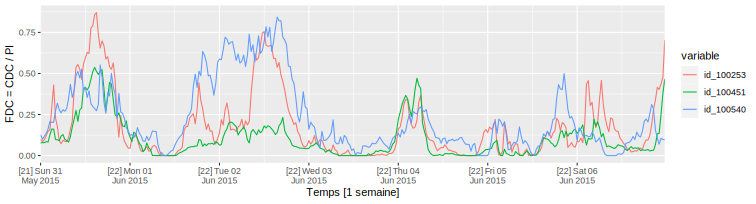
\includegraphics[width=0.75\textwidth]{Images/motivation/test__slice_graph__2015__id_1_2_3__week_1.jpg}
	}

	période : Juillet 2015

	\scalebox{0.7}{
		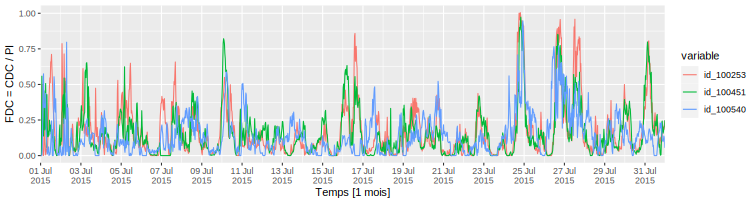
\includegraphics[width=0.75\textwidth]{Images/motivation/test__slice_graph__2015_07__id_1_2_3.jpg}
	}
	\caption{Courbes de charges éoliennes sur 3 premiers parcs éoliens}
	\label{fig:courbes_de_charge}
\end{figure}

Ainsi, les données qui sont traitées dans le cadre de ce stage sont, entre autres, des courbes de charge éoliennes observées chaque demie-heure. Le schéma d’observation est donc le 'common-design'. C'est-à-dire que les temps d'observations sont ici déterministes à intervalle de temps fixe.

\section{Difficulté de modélisation de la dynamique des données par un modèle de série temporelle classique}

Bien que la différenciation en analyse de séries temporelles soit une méthode efficace pour éliminer la tendance, qu'elle soit saisonnière ou non, permettant ainsi une bonne analyse des données; ces modèles présentent des limites en termes de prédiction à long terme, les rendant moins utiles lorsque l'objectif est de prédire à moyen ou long terme. De plus, ces modèles, ainsi que différents modèles de machine learning populaires, estiment les données courbe par courbe ce qui ne tire pas profit du fait que les observations aient une forme similaire entre les courbes.

\smallskip

Une première idée serait d'utiliser un modèle de série temporelle ARIMA afin de modéliser la dynamique des courbes de charge.


% \book{ \textbf{Un peu d'histoire sur les séries temporelles \ldots}        
\info{une grande partie des informations présentées dans cette section histoire provient de la référience ~\cite{time_series_brief_history} }


\smallskip

Parmi les étapes importantes du développement des séries temporelles, on peut noter l'article \emph{Time Series Analysis : Forecasting and Control} de Box et Jenkins (1970) qui introduit le modèle ARIMA et une approche aujourd'hui standarde d'évaluation du modèle à utiliser ainsi que son estimation. Ce développement est dû en grande partie à l'utilisation de telles données dans les secteurs économiques et des affaires afin de suivre l'évolution et la dynamique de différentes métriques

\smallskip

L'étude des séries temporelle a été divisée en l'étude du domaine fréquentiel, qui étudie le spectre des processus pour le décomposer en signaux principaux, et du domaine temporel, qui étudie les dépendances des indices temporels. L'utilisation de chacune des approches était sujet à débats mouvementés jusqu'aux alentours de l'an $2000$.

\smallskip

Le développement des capacités de calcul a été une révolution notamment pour l'identification des modèles (le critère AIC, l'estimation par vraissemblance dans les années $1980$, \ldots).
% modèles à espace d'états et le filtre de Kalman pour évaluer cette vraissemblance efficacement, MCMC, \ldots).

\smallskip

À partir des années $1980$, les modèles non linéaires émergent (ARCH par Engle, modèles à seuil \ldots) et trouvent application en économie notamment. Enfin l'étude multivariée (modèle VAR) fait surface dans les années 1980 par Christopher Sims~\cite[ \href{https://pubs.aeaweb.org/doi/pdf/10.1257/jep.15.4.101}{lien de l'article} ]{VAR_paper}

\smallskip

Une large partie de la théorie s'appuie notamment sur l'étude des racines de l'unité, en considérant un polynôme d'opérateur $P(B) = (I + \sum_k a_k B^k)$ à partir duquel les relations d'autocorrélations peuvent se ré-écrire.
% }


Bien que naturelle, l'utilisation d'un modèle ARIMA ne permet de modéliser la dynamique du phénomène étudié. En effet, la sélection d'un modèle ARIMA sur le critère du BIC sélectionnait, peu importe le parc éolien, un modèle auto-régressif d'ordre 0. Ainsi le modèle sélectionné considérait les irrégularités de la courbe de charge, dont on attend que le processus duquel elle est issue soit très irrégulier (de par sa complexité), comme étant du bruit. On en conclut que ces modèles peuvent ne pas capturer efficacement la structure complexe des données.

\section{Les données fonctionnelles comme solution à cette difficulté}

\subsubsection{définitions et propritétés informelles}


Commençons par introduire les données fonctionnelles de manière informelle afin de mieux intégrer la définition formelle, plus utile pour la manipulation.

Cette section regroupe l'ensemble des messages essentiels à retenir des données fonctionnelles pour la pratique, sans alourdir les notions avec des notations mathématiques. Le cadre formel sera traité juste après.

\begin{definition*}[données fonctionnelles — informel]
    Les données fonctionnelles sont des données dont les observations sont des fonctions, c'est-à-dire des courbes, des surfaces, des images, \, \dots
    
    i.e : toute donnée ayant une dépendance de type "relation fonctionnelle" avec un ou plusieurs paramètres.
\end{definition*}

Maintenant introduites, les théorèmes suivant permettent de manipuler ces données à la fois pour la théorie et la pratique :

\begin{thm*}[Karhunen-Loeve — informel]
    Il est possible pour une large classe de données fonctionnelles de les décomposer dans une base adaptée aux données (au sens de la covariance) que l'on appelle base ACP fonctionelle (FPCA).
\end{thm*}
\begin{proof}[\faCogs \, preuve informelle]
    La covariance est un opérateur bilinéaire symétrique défini positif, on peut donc appliquer le théorème de Mercer (équivalent du théorème spectral) qui nous donne une base orthonormale de $\mathds L^2$ sur laquelle on va décomposer notre processus \textbf{centré}.
\end{proof}
\begin{rem}
    La classe de fonctions pouvant être décomposées est large, puisqu'elle regroupe l'ensemble des processus qui nous intéressent la plus part du temps en tant que statisticien : celles qui sont à support sur un intervalle, admettant une covariance continue et finie sur le support.
\end{rem}
    
On en déduit que pour travailler avec des données fonctionnelles, il suffit de les décomposer dans la base ACP fonctionnelle puis de travailler sur les composantes de chaque élément de la base. On travaille désormais avec des réels et non plus des fonctions, ce qu'on aime manipuler. On peut alors faire de la statistique traditionnelle avec les outils que l'on connait.


\begin{propriete*}[intérêt de la base FPCA — informel]
    la base ACP fonctionnelle est la plus économe, c'est à dire qu'elle explique au mieux la covariance des données pour un nombre de composantes fixées, ce qui est utile car on ne sait manipuler numériquement que des objets de dimension finie.
\end{propriete*}

On a mentionné qu'il serait judicieux de lisser les observations en tenant compte de la régularité du processus dont est issu nos données. La question est désormais la suivante :

\question{
    Est-il possible de récupérer la régularité locale des trajectoires à partir des données ? Si oui, comment ?
}

C'est ce qu'affirme le théorème suivant à partir des travaux de Golovkine et al. ainsi que Maissoro-Patilea-Vimond (MPV) :

\begin{thm*}[Regularité locale — informel]
    Les données fonctionnelles permettent de récupérer la régularité locale des trajectoires. Les estimateurs définis \textbf{ponctuellement} convergent. 
\end{thm*}
\begin{rem}
    Les estimateurs sont définis à partir de l'espérance des incréments quadratiques du processus.
\end{rem}

Les motivations de l'obtention de la régularité étaient en partie de pouvoir mieux estimer la fonction moyenne du processus, ainsi que son opérateur de covariance. Ce qui est à la fois important pour l'analyse (via l'interprétation de la base ACP déterminée par la covariance) et pour la prédiction. On peut alors se demander si il existe des estimateurs de la moyenne et de la covariance prenant en compte la régularité locale. C'est ce qu'affirme les théorèmes suivants :

\warn{demander à Hassan la dernière version de son papier car la partie d estimation adaptative a beaucoup changé}

\begin{thm*}[Estimateurs de la moyenne et de la covariance — informel ~\cite{adaptative-estimation-irregular-mean-covariance}]
    Il est possible en lissant les observations par méthode à noyaux avec une largeur de bande \emph{spécifique à l'objet que l'on souhaite estimer}, de dériver des estimateurs de la moyenne et de la covariance qui convergent. 
    La largeur de bande optimale \emph{pour l'objet que l'on souhaite estimer} est celle qui minimise un risque qui effectue un compromis biais-variance, qui dépend de la régularité locale du processus, en pénalisant les largeurs de bande menant à des "trous" dans les fonctions lissées.
    On parle d'\emph{estimation adaptative}.
\end{thm*}

\begin{thm*}[expression de la largeur de bande optimale — informel ~\cite{adaptative-estimation-irregular-mean-covariance}]
    Sous certaines hypothèses de régularité du processus, et d'indépendance des temps observés, la largeur de bande optimale peut être approchée (avec forte probabilité de bonne approximation) par une expression ne dépendant que du nombre de courbes observées, du nombre moyen de temps observés par courbe, et de la régularité locale du processus. Ce biais de l'estimateur de la fonction moyenne est alors contrôlén fonction de ces mêmes quantités.

    Sous des hypothèses un peu plus fortes sur le nombre d'observations par courbe, et le nombre de courbe on dispose de résultats similaires pour l'estimateur de la covariance.
\end{thm*}


Enfin, on peut se demander ce qu'il en est des estimateurs dans le cadre où l'on dispose de la dépendance dans les données (ce qui est la cas pour les données éoliennes notamment). Ce cas est traîté par le théorème suivant dérivé par MPV :

\begin{thm*}

\end{thm*}



\subsubsection{définition formelle et premières propriétés}

\subsubsection{Définition formelle}

Pour éviter d'alourdir les notations, on se place dans le cas où les fonctions sont à valeurs dans $\mathds R$ et à support sur un intervalle fermé $I$ de $\mathds R$. Toutefois, on peut très bien considérer des fonctions à valeurs dans $\mathds R^d$ et à support sur un compact $K$ de $\mathds R^p$ sans perte de généralités.

\begin{definition}[données fonctionnelles ]

    On appelle données fonctionnelles, un échantillon $\famfinie x 1 n$ de fonctions continues $x_i : I \rightarrow \R d$ issues d'un processus $X$ défini comme ci-dessous :

    $$X : 
    \begin{array}{ccc}
        \Omega & \longrightarrow & \mathcal C(I, \mathds R)
        \\
        \omega & \longmapsto & X(\omega) = x 
    \end{array}
    $$

\end{definition}

\subsubsection{Résultats importants}

On énonce désormais le théorème central de l'analyse de données fonctionnelles qui n'est autre que la décomposition dans la base FPCA de notre processus.

\begin{rem}
    on notera que dans le cadre des données fonctionnelles, on ne travaille pas de façon générale avec la covariance :
    
    $$C_X : (s,t) \mapsto \esperance{ (X - \mu)(s) \cdot (X - \mu)(t) }$$
    
    On travaille plutôt avec l'\textbf{opérateur} covariance :
    $$f \mapsto \int\limits_I f(u)C_X(u, \cdot \,) \,du$$ 
    
    C'est parceque cet opérateur est linéaire continu (car Hilbert-Schmidt donc borné pour la norme d'opérateur) symétrique semi-défini positif (pour le produit scalaire de $\mathds L^2$) et que l'on peut donc en faire une décomposition spectrale sur une base orthonormale de vecteurs propres associés à des valeurs propres positives. Cette décomposition est à la base des approximations que le praticien effectuera ainsi qu'à la base de la dérivation de nombreux théorèmes et propriétés.
\end{rem}

\bigskip

Etant donné que l'on traîte des données fonctionnelles, on considère la géométrie usuelle de $\mathds L^2$ et on note ainsi 

$$\prodscalselon \cdot \cdot {\mathds L^2}: \begin{array}{ccc}
    \mathds L^2 \times \mathds L^2 & \longrightarrow & \mathds R
    \\
    (f,g) & \longmapsto & \int f(u)g(u) \, du 
\end{array}$$ 

le produit scalaire que l'on considère pour manipuler les données fonctionnelles.

% https://stackoverflow.com/a/4008463 : no page break
\begin{minipage}{\textwidth}
\begin{thm}[Karhunen-Loeve]
    \emph{référence :} ~\cite[pages : 238-239-241]{kokoszka2017introduction}

    \textbf{Hypothèses :}

    $$
    \boxed{
    \begin{array}{ll}
        \textsf{\faCaretSquareRight} & X \in \mathds L^2( \Omega, \mathcal C(I, \mathds R)) 
        \\ \\
        \textsf{\faCaretSquareRight} & \textsf{covariance : } C : \begin{array}{ccc}
            \mathds L^2( \Omega, \mathcal C(I, \mathds R)) & \longrightarrow & \mathcal C(I^2, \mathds R)
            \\
            X & \longmapsto & C_X
        \end{array}
        \\ \\
        & \textsf{ie : } C_X : (s, t) \mapsto C_X(s,t) \textsf{ est continue}
        \\ \\
        \textbf{\faIcon{asterisk}} & \textsf{opérateur covariance} \, c_X[ \, \cdot \, ] : \begin{array}{ccc}
            \mathcal C(I, \mathds R) & \longrightarrow & \mathcal C(I, \mathds R)
            \\
            f & \longmapsto & \int_I f(s) C_X(s, \cdot \, ) \, ds \end{array}
        \\\\
        \textsf{\faCaretSquareRight} & \textsf{valeurs propres ordonnées : } \forall p \geq 1, \lambda_{p+1} \leq \lambda_p \quad\quad \lambda_p, \lambda_{p+1} \in \operatorname{sp}(c_X)
        \\ \\
        \textbf{\faIcon{asterisk}} & \textsf{on pose } \overrightarrow{sp}_{\orthonormal}^{[1,p]}(c_X) \isdef \left\{ \phi_k \in \overrightarrow{sp}_{\orthonormal}( \, c_X \, ) \textsf{ associé à }  \lambda_k, k \in \intervaleint 1 p \, \right\}
    \end{array} 
    }
    $$

    \textbf{alors :}
    $$
    \boxed{
    \begin{array}{cc}
        \textsf{\faCaretSquareRight} & 

            \forall p \geq 1 
            \quad
            \argmin\limits_{u_k \in \mathcal C(I, \mathds R)} \mathds E \left\Vert X - \sum\limits_{k=1}^p \prodscalselon {X - \mu} {u_k} {\mathds L^2} u_k \right\Vert^2 = \overrightarrow{sp}_{\orthonormal}^{[1,p]}( \, c_X \, )

        \\
        \\
        \textsf{\faCaretSquareRight} & X = \mu + \sum\limits_{k=1}^{+\infty} \prodscal {X - \mu} {\phi_k} \phi_k
        \\
        &
        \\
         &\textsf{avec } \phi_k \in \overrightarrow{sp}_{\orthonormal}( \, c_X \, )
    \end{array}
    }
    $$

    \label{thm:KL}
\end{thm}
\end{minipage}

\begin{rem}
    pour pouvoir ordonner les valeurs propres dans l'ordre décroissant, et sélectionner les composantes principales les plus informatives, il faut pouvoir réarranger l'ordre de la somme. Pour cela il faut que les valeurs propres forment une famille sommable, une condition suffisante et souvent utilisée est que $\mathds E \Vert X \Vert^2 < \infty$ 
\end{rem}

\begin{rem}
    la propriété de la section précédente sur l'aspect économe de la base FPCA découle directement de l'assertion $\forall p \geq 1 
    \quad
    \argmin\limits_{u_k \in \mathcal C(I, \mathds R)} \mathds E \left\Vert X - \sum\limits_{k=1}^p \prodscal {X - \mu} {u_k} u_k \right\Vert^2 = \overrightarrow{sp}_{\orthonormal}^{[1,p]}( \, c_X \, )$ dans le théorème de Karhunen-Loeve.
\end{rem}




\section{Importance de l'estimation de la régularité}

Comme mentionné auparavant, la production électrique est un phénomène très irrégulier [figure ~\ref{fig:courbes_de_charge} étant influencé par la consommation, la météo, etc. Par conséquent, la prévision de ces courbes de charge doit prendre en compte la nature fondamentalement irrégulière du phénomène afin de proprement le modéliser et, en définitive, mieux le prédire. 
Ce qui est notamment contraire à de nombreux modèles populaires parmi les statisticiens qui utilisent des fonctions de classe $\mathcal C^2$ pour lisser les points observés en données fonctionnelles, ce qui limite la prédiction à des courbes de nature $\mathcal C^2$. 
Cela est d'autant plus critique lorsque l'on cherche à estimer le processus moyen ou l'opérateur de covariance du processus, car ces derniers sont estimés à partir des courbes lissées. 
Le lissage détruit alors toute l'information irrégulière si elle n'est pas prise en compte et ainsi impacte significativement l'estimation des objets qui nous intéressent en tant que statisticien.

\begin{figure}[H]
	\centering
	\begin{tikzpicture}
		\pgfmathsetmacro{\pgfdeltavalue}{0.25}
		\pgfmathsetmacro{\pgftvalue}{0.4}
		\pgfmathsetmacro{\pgfarrowheight}{-0.25}
		\pgfmathsetmacro{\pgfarrowfrom}{\pgftvalue - \pgfdeltavalue/2}
		\pgfmathsetmacro{\pgfarrowto}{\pgftvalue + \pgfdeltavalue/2}
		\begin{axis}[axis lines=middle,
				xmin=0, xmax=1,
				ymin=-0.4, ymax=0.4,
				axis equal image,
				ytick=\empty,
				xtick=\empty,
				legend style={at={(0.5,-0.15)},anchor=north east},
				legend entries={$\mathcal C^0$, $\mathcal C^2$}
			]
			\addplot [flatuicolors_green, samples=800, domain=0:1.1] {weierstrass(2*x,2,15)};

			\addplot [flatuicolors_orange, samples=200, domain=0:1.1] {0.37*sin(2*3.1215*deg(x))};

		\end{axis}
	\end{tikzpicture}
	\label{fig:continu_vs_c_deux}
	\caption{Comparaison entre une courbe $\mathcal C^2$ et une courbe non dérivable}
\end{figure}


Il est ainsi important pour des phénomènes de nature irrégulière de ne pas négliger des précautions lors du lissage afin de ne pas perdre l'information irrégulière. L'idée est donc d'estimer dans un premier temps la régularité de notre processus afin de lisser nos données de manière adaptée. Il est alors possible prédire des valeurs non observées tout en préservant les informations irrégulières. Cela permet enfin d'obtenir une bonne estimation du processus moyen et de l'opérateur de covariance. L'approche fonctionnelle est clé dans l'estimation de cette régularité, car c'est la \textbf{réplication de courbes} de même nature qui permet in-fine d'\textbf{estimer la régularité} du phénomène, et il est donc important de bien savoir l'estimer.

\section{Importance du choix du voisinage utilisé pour l'estimation de la régularité}

\question{ L'estimation de la régularité des trajectoires est certes importante mais comment l'estime-t-on en pratique ? }


% TODO : ❌ PEUT SE FAIRE MEME EN DEPENDANCE FORTE
Dans le cadre de données avec dépendance faible, il est possible d'estimer la régularité locale du processus ponctuellement en utilisant les informations d'un voisinage arbitrairement donné\footnote{L'étude de la convergence des estimateurs des paramètres de régularité locale a été établie par Golovkine et al. ainsi que Maissoro-Patilea-Vimond\footnote{qui seront désormais mentionnés par \og MPV \fg} \cite{golovkineRegularityOnlineEstimationNoisyCurve,maissoro-SmoothnessFTSweakDep}.}. Cependant bien que l'estimateur soit convergent en utilisant un voisinage quelconque, il n'est pas spécifié de quelle taille devrait être ce voisinage pour avoir une bonne estimation des paramètres de régularité locale\footnote{On entend par bonne estimation une estimation qui comporte les caractéristiques suivantes : une bonne vitesse de convergence, un compromis biais-variance adapté à l'application souhaitée de notre estimateur}. On appelle le diamètre du voisinage que l'on considère pour effectuer les calculs \og$\Delta$\fg.

\question{Si la convergence des estimateurs est déjà déterminée pour un $\Delta$ donné arbitraire, pourquoi ne pas simplement en prendre un de façon arbitraire ?}

Choisir un diamètre de voisinage non approprié mènerait à utiliser des informations non pertinentes pour estimer la régularité car celle-ci peut être variable sur l'ensemble de la trajectoire. De plus, il est naturel de penser que différents niveaux de régularités requièrent de regarder des informations d'une proximité différente.\footnote{Considérer $|x-x_0| = \Delta$ dans la définition de la régularité que l'on considère en \ref{annexe:regularite-def} } On introduirait alors un biais significatif dans l'estimation des paramètres de régularité locale, dont on a vu qu'il était important de bien estimer.


\section{Objectif du stage}

Choisir le bon diamètre du voisinage $(\Delta)$ que l'on considère pour estimer la régularité locale est donc un problème important, et c'est ce que l'on va étudier lors de ce stage. L'objectif est d'obtenir une procédure de détermination du $\Delta$ que le praticien devra choisir pour l'estimation de la régularité locale en fonction de quantités facilement estimables, comme nombre moyen de points observés par courbe par exemple.

Pour cela, on simulera 200 réplications indépendantes de monte-carlo d'un modèle auto-régressif fonctionnel dont les bruits blancs sont des mouvements browniens multi-fractionnaires de régularité variable connue. Les estimateurs de régularité fournis par MPV ~\cite{maissoro-SmoothnessFTSweakDep} seront ensuite utilisés pour estimer la régularité (connue) de ces courbes. La procédure de sélection du $\Delta$ sera alors déterminée en s'appuyant sur l'analyse du comportement d'un risque d'estimation de la régularité en fonction du $\Delta$ choisi. Enfin la procédure déterminée sera testée sur les données simulées avant d'être appliquée sur des données réelles pour estimer de façon adaptative la fonction moyenne.
